\section{Kabinet}

For at øge SPL for højtalerens resonansfrekvens, sættes højtaleren i et kabinet der er designet til formålet.
Kabinettets ønskede volumen kan findes i databladet for højtaleren\cite{FW168} som ækvivalent volumen $V_{as} = 16.5L$. Ved denne højtalervolumen vil resonansfrekvensen $f_s$ dog øges med ca. $41\%$ da den indskudte masse af luften vil give højtaleren mindre bevægelsesfrihed. Dvs $45Hz\cdot1.45=65.25Hz$

Med et basreflekskabinet vil man kunne sænke\fxnote{ikke helt rigtigt LS} resonansfrekvensen igen da man med luftmassen i porten, vil skabe en fjedervirkning som sammen med kabinettets indespærrede luft kan afstemmes til en given resonansfrekvens. For størst effekt, bør denne resonans afstemmes til højtalerens resonansfrekvens $f_s = 45Hz$.

Portens resonansfrekvens findes med ligning \ref{lig:fport}
\begin{equation}\label{lig:fport}
f_{port}=\frac{1}{2 \pi \sqrt{M_{AP} C_{AB}}}
\end{equation}
Hvor $M_{AP}$ er portens akustiske luftmasse og $C_{AB}$ er massen af kabinettets akustiske luftvolumen.
\begin{equation}\label{lig:CAB}
C_{AB}=\frac{V_{as}}{\rho c^2}
	\end{equation}
	Hvor luftens massefylde er $\rho=1.18 \frac{kg}{m^3}$ 
\begin{equation}\label{lig:MAP}
M_{AP}=\frac{\rho}{S_P} (L_P+1.5\sqrt{\frac{S_P}{\pi}})
\end{equation}	
Hvor portens areal her er bestemt til $S_P=2cm^2$

Indsætter man ligning \ref{lig:MAP} i ligning \ref{lig:fport} og solver for $f_{port}=45Hz$ får man portens længde til 13.91cm (Realiseret med 15cm)

\fxnote{Laves også med mellem og kort rør + dermed ændring af luftvolummet.}

Resonansfrekvensen for kabinettet udregnes i ligning \ref{lig:fckabinet}, hvilket er tæt på de $41\%$ ekstra.
\begin{equation}\label{lig:fckabinet}
f_{kabinet}=\frac{1}{2 \pi \sqrt{M_{AS} \cdot C_{AS}||C_{AB}}} = 64.57Hz
\end{equation}
\begin{figure}[H]
	\centering
	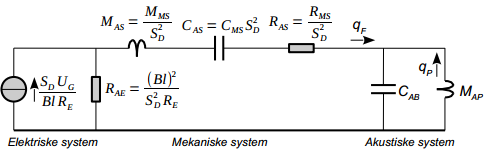
\includegraphics[width=\textwidth]{Pics/Akustisk_basrefleks_model.PNG}
	\label{fig:BR_a_Model}
	\caption{Akustisk model for højtaler i basreflekskabinet \cite{Elektroakustik}} 
\end{figure}